% IT Ethics Lecture 2: Virtues in the Age of Social Media and AI
% Brendan Shea, PhD
% Rochester Community and Technical College

\documentclass[aspectratio=169]{beamer}

% Theme and colors
\usetheme{Madrid}
\usecolortheme{whale}
\setbeamertemplate{navigation symbols}{}
\setbeamertemplate{footline}[frame number]

% Packages
\usepackage[utf8]{inputenc}
\usepackage[T1]{fontenc}
\usepackage{graphicx}
\usepackage{booktabs}
\usepackage{array}
\usepackage{multirow}
\usepackage{hyperref}
\usepackage{csquotes}

% TikZ and libraries
\usepackage{tikz}
\usetikzlibrary{shapes.geometric, arrows.meta, positioning, calc, backgrounds, fit, decorations.pathreplacing, shadows, mindmap, trees}

% Custom colors
\definecolor{primaryblue}{RGB}{0,74,124}
\definecolor{accentorange}{RGB}{230,126,34}
\definecolor{lightgray}{RGB}{245,245,245}
\definecolor{darktext}{RGB}{44,62,80}


% Title information
\title[IT Ethics: Lecture 2]{Virtues in the Age of Social Media and AI}
\subtitle{Character, Technology, and Human Flourishing}
\author{Brendan Shea, PhD}
\institute[RCTC]{Rochester Community and Technical College}
\date{Spring 2026}

\begin{document}

%------------------------------------------------------
% SLIDE 1: Title Slide
%------------------------------------------------------
\begin{frame}
\titlepage
\end{frame}

%------------------------------------------------------
% SLIDE 2: Recap: Five Information Technology Revolutions
%------------------------------------------------------
\begin{frame}{Recap: Five Information Technology Revolutions}
    \begin{itemize}
        \item In Lecture 1, we traced five major \textbf{information technology revolutions} that transformed how humans create, store, and share knowledge.
        \item Each revolution changed not just \textit{what} we can do with information, but \textit{who} controls it and \textit{how} it shapes society.
        \item We saw recurring patterns: promises of democratization, fears of lost skills, debates over gatekeeping, and unintended consequences.
        \item Today we focus on what comes \textit{after} Web 1.0: the rise of social media, algorithmic platforms, and artificial intelligence.
    \end{itemize}
    
    \vspace{0.3em}
    
    \begin{center}
    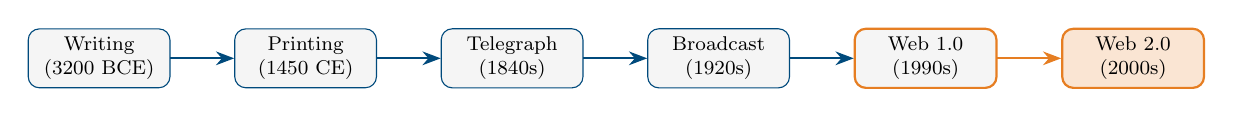
\begin{tikzpicture}[
        node distance=0.9cm,
        every node/.style={font=\small},
        scale =0.9,
        transform shape,
        box/.style={rectangle, draw=primaryblue, fill=lightgray, rounded corners, minimum width=2cm, minimum height=0.7cm, align=center, font=\footnotesize}
    ]
        \node[box] (writing) {Writing\\(3200 BCE)};
        \node[box, right=of writing] (printing) {Printing\\(1450 CE)};
        \node[box, right=of printing] (telegraph) {Telegraph\\(1840s)};
        \node[box, right=of telegraph] (broadcast) {Broadcast\\(1920s)};
        \node[box, right=of broadcast, draw=accentorange, thick] (web) {Web 1.0\\(1990s)};
        \node[box, right=of web, draw=accentorange, fill=accentorange!20, thick] (web2) {Web 2.0\\(2000s)};
        
        \draw[-{Stealth}, thick, primaryblue] (writing) -- (printing);
        \draw[-{Stealth}, thick, primaryblue] (printing) -- (telegraph);
        \draw[-{Stealth}, thick, primaryblue] (telegraph) -- (broadcast);
        \draw[-{Stealth}, thick, primaryblue] (broadcast) -- (web);
        \draw[-{Stealth}, thick, accentorange] (web) -- (web2);
    \end{tikzpicture}
    \end{center}
\end{frame}

%------------------------------------------------------
% SLIDE 3: From Web 1.0 to Web 2.0
%------------------------------------------------------
\begin{frame}{From Web 1.0 to Web 2.0}
    \begin{itemize}
        \item \textbf{Web 1.0} (roughly 1991--2004) was primarily a ``read-only'' web: static pages created by webmasters, organized by directories like Yahoo, with users as passive consumers.
        \item \textbf{Web 2.0} (2004--present) transformed the web into a ``read-write'' platform where ordinary users generate content through blogs, social networks, and video sharing.
        \item This shift moved power from professional publishers to platforms that aggregate user-generated content---but also concentrated power in new ways.
        \item The term ``Web 2.0'' was popularized by Tim O'Reilly in 2004 to describe this architectural and cultural transformation.
    \end{itemize}
    
    \vspace{0.2em}
    
    \begin{center}
    \renewcommand{\arraystretch}{1.2}
    \begin{tabular}{>{\raggedright}p{3.5cm} >{\raggedright}p{4.5cm} >{\raggedright\arraybackslash}p{4.5cm}}
        \toprule
        \textbf{Feature} & \textbf{Web 1.0} & \textbf{Web 2.0} \\
        \midrule
        Content Creation & Webmasters, companies & Anyone with an account \\
        User Role & Consumer (read) & Producer (read/write) \\
        Organization & Directories, portals & Search, social feeds \\
        Examples & GeoCities, AOL & Facebook, YouTube, Wikipedia \\
        \bottomrule
    \end{tabular}
    \end{center}
\end{frame}

%------------------------------------------------------
% SLIDE 4: The Architecture of Web 2.0
%------------------------------------------------------
\begin{frame}{The Architecture of Web 2.0}
    \begin{itemize}
        \item \textbf{Platforms} are digital intermediaries that connect users, content creators, and advertisers---they don't create content but profit from hosting it.
        \item \textbf{User-generated content} means the platform's value comes from what users post: status updates, photos, videos, reviews, and comments.
        \item \textbf{Social graphs} map relationships between users, enabling features like friend recommendations, news feeds, and targeted advertising.
        \item \textbf{Network effects} make platforms more valuable as more people join---your friends are on Facebook, so you join Facebook, making it more valuable for others.
    \end{itemize}
    
    \vspace{0.2em}
    
    \begin{center}
    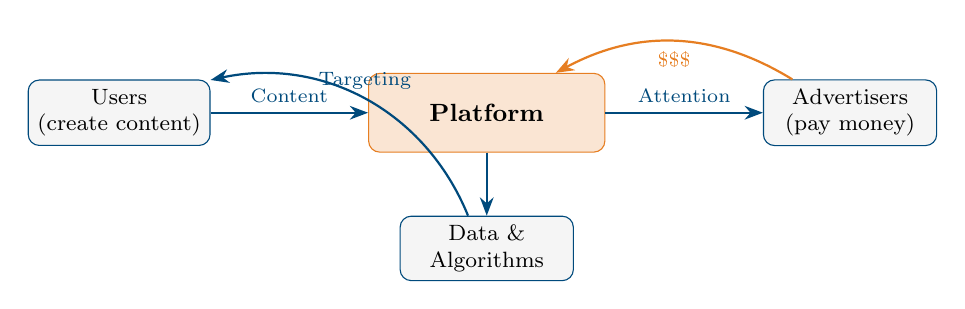
\begin{tikzpicture}[
        node distance=1.5cm,
        box/.style={rectangle, draw=primaryblue, fill=lightgray, rounded corners, minimum width=2.2cm, minimum height=0.8cm, align=center, font=\footnotesize},
        platform/.style={rectangle, draw=accentorange, fill=accentorange!20, rounded corners, minimum width=3cm, minimum height=1cm, align=center, font=\small\bfseries}
    ]
        \node[box] (users) {Users\\(create content)};
        \node[platform, right=2cm of users] (platform) {Platform};
        \node[box, right=2cm of platform] (advertisers) {Advertisers\\(pay money)};
        \node[box, below=0.8cm of platform] (data) {Data \&\\Algorithms};
        
        \draw[-{Stealth}, thick, primaryblue] (users) -- node[above, font=\scriptsize] {Content} (platform);
        \draw[-{Stealth}, thick, primaryblue] (platform) -- node[above, font=\scriptsize] {Attention} (advertisers);
        \draw[-{Stealth}, thick, accentorange] (advertisers) to[bend right=30] node[below, font=\scriptsize] {\$\$\$} (platform);
        \draw[-{Stealth}, thick, primaryblue] (platform) -- (data);
        \draw[-{Stealth}, thick, primaryblue] (data) to[bend right=40] node[above, font=\scriptsize] {Targeting} (users);
    \end{tikzpicture}
    \end{center}
\end{frame}

%------------------------------------------------------
% SLIDE 5: The Attention Economy and the Infosphere
%------------------------------------------------------
\begin{frame}{The Attention Economy and the Infosphere}
    \begin{itemize}
        \item Web 2.0 platforms are free to use because \textbf{you are not the customer---you are the product}; your attention is sold to advertisers.
        \item The \textbf{attention economy} treats human attention as a scarce resource to be captured, measured, and monetized through engagement metrics.
        \item Philosopher Luciano Floridi argues we now live in an \textbf{infosphere}---an environment where the boundaries between online and offline life have dissolved.
        \item In this infosphere, we have become \textbf{inforgs} (informational organisms): beings whose identities, relationships, and choices are increasingly mediated by digital information.
    \end{itemize}
    
    \vspace{0.3em}
    
    \begin{alertblock}{The Business Model}
        ``If you're not paying for the product, you are the product.'' Platforms maximize \textbf{engagement} (time on site, clicks, shares) because more engagement means more advertising revenue---regardless of whether that engagement benefits users.
    \end{alertblock}
\end{frame}

%------------------------------------------------------
% SLIDE 6: Algorithmic Feeds and Filter Bubbles
%------------------------------------------------------
\begin{frame}{Algorithmic Feeds and Filter Bubbles}
    \begin{itemize}
        \item \textbf{Algorithmic feeds} replaced chronological timelines around 2009--2016; platforms now decide what you see based on predicted engagement.
        \item \textbf{Filter bubbles} (Eli Pariser, 2011) occur when algorithms show you content similar to what you've engaged with before, narrowing your information diet.
        \item \textbf{Echo chambers} form when users primarily encounter views that reinforce their existing beliefs, making opposing perspectives seem alien or extreme.
        \item These systems optimize for \textit{engagement}, not truth, understanding, or wellbeing---outrage and controversy often generate more clicks than nuance.
    \end{itemize}
    
    \vspace{0.2em}
    
    \begin{center}
    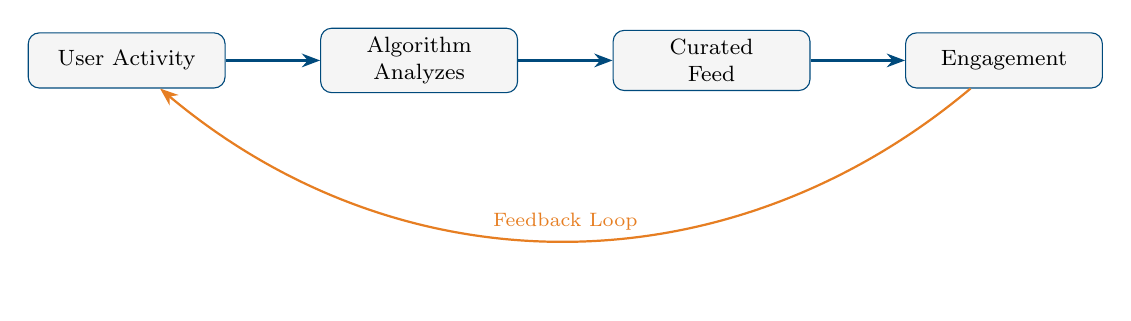
\begin{tikzpicture}[
        node distance=0.8cm,
        box/.style={rectangle, draw=primaryblue, fill=lightgray, rounded corners, minimum width=2.5cm, minimum height=0.7cm, align=center, font=\footnotesize},
        arrow/.style={-{Stealth}, thick, primaryblue}
    ]
        \node[box] (user) {User Activity};
        \node[box, right=1.2cm of user] (algorithm) {Algorithm\\Analyzes};
        \node[box, right=1.2cm of algorithm] (feed) {Curated\\Feed};
        \node[box, right=1.2cm of feed] (engage) {Engagement};
        
        \draw[arrow] (user) -- (algorithm);
        \draw[arrow] (algorithm) -- (feed);
        \draw[arrow] (feed) -- (engage);
        \draw[arrow, accentorange, bend left=40] (engage) to node[above, font=\scriptsize] {Feedback Loop} (user);
    \end{tikzpicture}
    \end{center}
\end{frame}

%------------------------------------------------------
% SLIDE 7: From Social Media to AI: A Continuous Story
%------------------------------------------------------
\begin{frame}{From Social Media to AI: A Continuous Story}
    \begin{itemize}
        \item This lecture examines social media and AI together because they are \textbf{not separate phenomena}---AI is the next chapter in the same story.
        \item Social media trained us to seek validation from likes, to curate personas, and to prefer mediated interaction over face-to-face conversation.
        \item Generative AI (ChatGPT, 2022) extends these patterns: now we can have ``relationships'' with systems that simulate understanding without possessing it.
        \item The thinkers we'll study---Vallor, Turkle, Haidt, Floridi---have all extended their frameworks from social media to AI, seeing continuity rather than rupture.
    \end{itemize}
    
    \vspace{0.3em}
    
    \begin{block}{Sherry Turkle, \textit{Reclaiming Conversation} (2024 Preface)}
        ``Social media was our gateway drug to conversations with machines.''
    \end{block}
\end{frame}

%------------------------------------------------------
% SLIDE 8: Discussion Questions: Web 2.0 and the Infosphere
%------------------------------------------------------
\begin{frame}{Discussion Questions: Web 2.0 and the Infosphere}
    \begin{enumerate}
        \item  You get free access to powerful platforms; they get your attention data. Is this a fair exchange? Who benefits more?
        
        \vspace{0.5em}
        
        \item  How would you know if you were in a filter bubble? What steps, if any, do you take to encounter perspectives different from your own?
        
        \vspace{0.5em}
        
        \item  Floridi says we've become ``informational organisms'' whose identities are partly constituted by our digital presence. Does this match your experience? Is this troubling or simply the new normal?
        
        \vspace{0.5em}
        
        \item  Turkle suggests social media prepared us for AI relationships. Do you see connections between how you use social media and how you might interact with AI assistants?
    \end{enumerate}
\end{frame}

%------------------------------------------------------
% SLIDE 9: What Is Virtue Ethics?
%------------------------------------------------------
\begin{frame}{What Is Virtue Ethics?}
    \begin{itemize}
        \item \textbf{Virtue ethics} is a moral framework that focuses on \textit{character}---the kind of person you are---rather than on rules or consequences alone.
        \item While \textbf{deontology} asks ``What rules should I follow?'' and \textbf{consequentialism} asks ``What outcome should I produce?'', virtue ethics asks ``What kind of person should I become?''
        \item A \textbf{virtue} is an excellent trait of character---like honesty, courage, or compassion---that enables a person to live well and flourish.
        \item Virtue ethics emphasizes that good actions flow from good character, which is developed through \textbf{practice and habituation} over time.
    \end{itemize}
    
    \vspace{0.2em}
    
    \begin{center}
    \renewcommand{\arraystretch}{1.2}
    \begin{tabular}{>{\raggedright}p{3cm} >{\raggedright}p{4cm} >{\raggedright\arraybackslash}p{4.5cm}}
        \toprule
        \textbf{Approach} & \textbf{Central Question} & \textbf{Key Concept} \\
        \midrule
        Deontology & What is my duty? & Rules, obligations \\
        Consequentialism & What produces the best outcome? & Utility, welfare \\
        \textbf{Virtue Ethics} & \textbf{What kind of person should I be?} & \textbf{Character, flourishing} \\
        \bottomrule
    \end{tabular}
    \end{center}
\end{frame}

%------------------------------------------------------
% SLIDE 10: Aristotle and Eudaimonia
%------------------------------------------------------
\begin{frame}{Aristotle and Eudaimonia}
    \begin{itemize}
        \item \textbf{Aristotle} (384--322 BCE) is the founding figure of Western virtue ethics; his \textit{Nicomachean Ethics} remains the most influential text in the tradition.
        \item Aristotle argues that all human action aims at some \textbf{good}, and the highest good is \textbf{eudaimonia}---often translated as ``happiness'' but better understood as ``flourishing'' or ``living well.''
        \item Eudaimonia is not a feeling but an \textbf{activity}---it is achieved by living in accordance with virtue throughout a complete life.
        \item For Aristotle, humans flourish by exercising their distinctive capacity: \textbf{reason}---both in thinking well and in governing emotions and desires wisely.
    \end{itemize}
    
    \vspace{0.3em}
    
    \begin{block}{Aristotle, \textit{Nicomachean Ethics} (c. 340 BCE)}
        ``Happiness [eudaimonia] is an activity of the soul in accordance with virtue, and if there are several virtues, in accordance with the best and most complete.''
    \end{block}
\end{frame}

%------------------------------------------------------
% SLIDE 11: Aristotle's Doctrine of the Mean
%------------------------------------------------------
\begin{frame}{Aristotle's Doctrine of the Mean}
    \begin{itemize}
        \item Aristotle's \textbf{doctrine of the mean} holds that each virtue is a balanced middle point between two extremes: one of excess and one of deficiency.
        \item The mean is not a mathematical average but the \textbf{right amount} for this person, in this situation---it requires judgment, not calculation.
        \item Finding the mean requires \textbf{practical wisdom} (phronesis): the ability to perceive what virtue requires in particular circumstances.
        \item This framework suggests that virtuous technology use involves finding balance---neither total abstinence nor unreflective immersion.
    \end{itemize}
    
    \vspace{0.2em}
    
    \begin{center}
    \renewcommand{\arraystretch}{1.15}
    \begin{tabular}{>{\raggedright}p{3cm} >{\centering}p{3cm} >{\raggedright\arraybackslash}p{3cm}}
        \toprule
        \textbf{Deficiency} & \textbf{Virtue (Mean)} & \textbf{Excess} \\
        \midrule
        Cowardice & \textbf{Courage} & Recklessness \\
        Stinginess & \textbf{Generosity} & Wastefulness \\
        Self-deprecation & \textbf{Truthfulness} & Boastfulness \\
        Boorishness & \textbf{Wit} & Buffoonery \\
        \bottomrule
    \end{tabular}
    \end{center}
\end{frame}

%------------------------------------------------------
% SLIDE 12: Habituation and Practical Wisdom
%------------------------------------------------------
\begin{frame}{Habituation and Practical Wisdom}
    \begin{itemize}
        \item Aristotle insists that virtues are not innate---we are not born courageous or just---but are developed through \textbf{habituation}: repeated practice until virtuous action becomes second nature.
        \item ``We become just by doing just acts, temperate by doing temperate acts, brave by doing brave acts''---character is formed by what we \textit{repeatedly do}.
        \item \textbf{Phronesis} (practical wisdom) is the master virtue: the capacity to discern the right action in particular circumstances, balancing competing considerations.
        \item This has profound implications for technology: our digital habits shape our character, and we need practical wisdom to navigate novel situations that Aristotle never imagined.
    \end{itemize}
    
    \vspace{0.2em}
    
    \begin{exampleblock}{Technology Application}
        If virtues are formed by habits, then our daily technology practices---checking phones first thing in the morning, scrolling before sleep, responding instantly to notifications---are shaping who we become. What character traits do these habits cultivate?
    \end{exampleblock}
\end{frame}

%------------------------------------------------------
% SLIDE 13: Confucian Virtue Ethics
%------------------------------------------------------
\begin{frame}{Confucian Virtue Ethics}
    \begin{itemize}
        \item \textbf{Confucius} (551--479 BCE) developed a virtue tradition in China contemporaneous with Greek philosophy, emphasizing social relationships and moral cultivation.
        \item The central virtue is \textbf{ren}---variously translated as ``humaneness,'' ``benevolence,'' or ``human-heartedness''---the quality of caring appropriately for others.
        \item \textbf{Li} refers to ritual propriety: the customs, manners, and social forms through which we express respect and maintain harmonious relationships.
        \item The goal is to become a \textbf{junzi}---an ``exemplary person'' or ``gentleman''---who cultivates virtue and serves as a moral model for others.
    \end{itemize}
    
    \vspace{0.3em}
    
    \begin{block}{Confucius, \textit{Analects} 12.2}
        ``Do not do to others what you would not want done to yourself.''
    \end{block}
\end{frame}

%------------------------------------------------------
% SLIDE 14: Confucianism: Relationships and Moral Cultivation
%------------------------------------------------------
\begin{frame}{Confucianism: Relationships and Moral Cultivation}
    \begin{columns}[T]
        \begin{column}{0.55\textwidth}
            \begin{itemize}
                \small
                \item Unlike Aristotle's focus on individual flourishing, Confucian ethics is fundamentally \textbf{relational}---virtue is expressed through our roles as children, parents, friends, citizens, and colleagues.
                \item The \textbf{Five Relationships} (wulun) define core moral bonds: parent-child, ruler-subject, husband-wife, elder-younger sibling, and friend-friend.
                \item Moral development requires \textbf{self-cultivation} (xiuyang): continuous effort to refine one's character through study, reflection, and practice.
                \item This relational focus raises important questions: How do digital technologies affect our ability to fulfill our roles and obligations to others?
            \end{itemize}
        \end{column}
        
        \begin{column}{0.4\textwidth}
            \begin{center}
            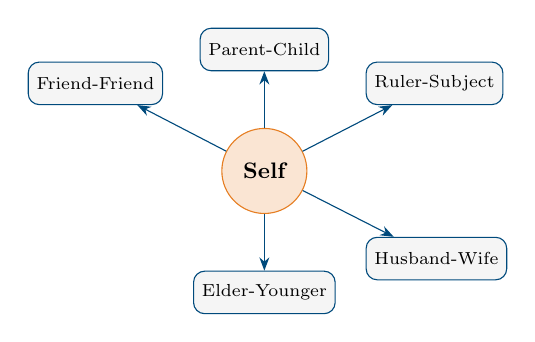
\begin{tikzpicture}[
                scale=0.9,
                transform shape,
                node distance=1cm,
                center/.style={circle, draw=accentorange, fill=accentorange!20, minimum size=1.2cm, font=\small\bfseries},
                relation/.style={rectangle, draw=primaryblue, fill=lightgray, rounded corners, minimum width=1.8cm, minimum height=0.6cm, font=\scriptsize, align=center}
            ]
                \node[center] (self) {Self};
                \node[relation, above=0.8cm of self] (parent) {Parent-Child};
                \node[relation, above right=0.5cm and 1cm of self] (ruler) {Ruler-Subject};
                \node[relation, below right=0.5cm and 1cm of self] (spouse) {Husband-Wife};
                \node[relation, below=0.8cm of self] (sibling) {Elder-Younger};
                \node[relation, above left=0.5cm and 1cm of self] (friend) {Friend-Friend};
                
                \draw[-{Stealth}, primaryblue] (self) -- (parent);
                \draw[-{Stealth}, primaryblue] (self) -- (ruler);
                \draw[-{Stealth}, primaryblue] (self) -- (spouse);
                \draw[-{Stealth}, primaryblue] (self) -- (sibling);
                \draw[-{Stealth}, primaryblue] (self) -- (friend);
            \end{tikzpicture}
            \end{center}
        \end{column}
    \end{columns}
\end{frame}

%------------------------------------------------------
% SLIDE 15: Religious Virtue Traditions
%------------------------------------------------------
\begin{frame}{Religious Virtue Traditions}
    \begin{itemize}
        \item Most world religions include robust virtue traditions that overlap with and extend philosophical approaches to character ethics.
        \item \textbf{Christianity} distinguishes cardinal virtues (prudence, justice, fortitude, temperance) from theological virtues (faith, hope, charity/love) that require divine grace.
        \item \textbf{Islam} emphasizes virtues like \textbf{taqwa} (God-consciousness), \textbf{sabr} (patience), and \textbf{ihsan} (excellence in worship and conduct toward others).
        \item \textbf{Buddhism}'s Noble Eightfold Path cultivates virtues of wisdom (right view, intention), ethical conduct (right speech, action, livelihood), and mental discipline (right effort, mindfulness, concentration).
    \end{itemize}
    
    \vspace{0.2em}
    
    \begin{center}
        \scriptsize
    \renewcommand{\arraystretch}{1.15}
    \begin{tabular}{>{\raggedright}p{2.5cm} >{\raggedright\arraybackslash}p{9cm}}
        \toprule
        \textbf{Tradition} & \textbf{Key Virtues} \\
        \midrule
        Christianity & Prudence, justice, fortitude, temperance; faith, hope, love \\
        Islam & Taqwa (consciousness), sabr (patience), ihsan (excellence) \\
        Buddhism & Right speech, right action, right mindfulness \\
        Judaism & Tzedakah (justice/charity), chesed (loving-kindness), emet (truth) \\
        \bottomrule
    \end{tabular}
    \end{center}
\end{frame}

%------------------------------------------------------
% SLIDE 16: Care Ethics and Relationships
%------------------------------------------------------
\begin{frame}{Care Ethics and Relationships}
    \begin{itemize}
        \item \textbf{Care ethics} emerged in the 1980s from feminist philosophy, emphasizing relationships, context, and emotional responsiveness over abstract universal rules.
        \item \textbf{Carol Gilligan} argued that traditional ethics privileged ``justice reasoning'' (rights, rules) over ``care reasoning'' (relationships, responsibilities, responsiveness to particular others).
        \item \textbf{Nel Noddings} developed care ethics as a complete moral theory: the fundamental moral relation is the caring encounter between ``one-caring'' and ``cared-for.''
        \item Care ethics asks: What do \textit{these particular people} in \textit{this relationship} need from each other?---a question algorithms cannot answer.
    \end{itemize}
    
    \vspace{0.3em}
    
    \begin{exampleblock}{Technology Application}
        Care ethics highlights what's lost when relationships are mediated by screens: the ability to perceive subtle cues, respond to unspoken needs, and be physically present. Can we truly ``care'' through a platform optimized for engagement metrics?
    \end{exampleblock}
\end{frame}

%------------------------------------------------------
% SLIDE 17: Communitarian Political Philosophy
%------------------------------------------------------
\begin{frame}{Communitarian Political Philosophy}
    \begin{itemize}
        \item \textbf{Communitarianism} emerged in the 1980s as a critique of liberal individualism, arguing that identity and morality are shaped by communities, traditions, and shared practices.
        \item \textbf{Alasdair MacIntyre}'s \textit{After Virtue} (1981) argues that modern society has lost a coherent moral framework; we need to recover virtue within living traditions and practices.
        \item \textbf{Michael Sandel} criticizes the liberal idea of the ``unencumbered self''---we are not abstract individuals but members of families, communities, and nations that shape who we are.
        \item \textbf{Charles Taylor} emphasizes that humans are ``self-interpreting animals'' who need shared frameworks of meaning to understand what makes life worthwhile.
    \end{itemize}
    
    \vspace{0.3em}
    
    \begin{block}{Alasdair MacIntyre, \textit{After Virtue} (1981)}
        ``I can only answer the question `What am I to do?' if I can answer the prior question `Of what story or stories do I find myself a part?'\,''
    \end{block}
\end{frame}

%------------------------------------------------------
% SLIDE 18: Practices, Communities, and Virtues
%------------------------------------------------------
\begin{frame}{Practices, Communities, and Virtues}
    \begin{itemize}
        \item MacIntyre defines a \textbf{practice} as a cooperative activity with internal goods (excellence) and external goods (money, fame)---examples include medicine, teaching, chess, and farming.
        \item Virtues are the qualities needed to achieve the \textbf{internal goods} of practices: a good doctor needs honesty, compassion, and practical wisdom, not just technical skill.
        \item Practices are sustained by \textbf{institutions} (hospitals, universities, guilds), but institutions tend to prioritize external goods and can corrupt practices.
        \item This framework raises questions: Is social media use a practice? What internal goods might it have? How do platform business models affect those goods?
    \end{itemize}
    
    \vspace{0.2em}
    
    \begin{center}
    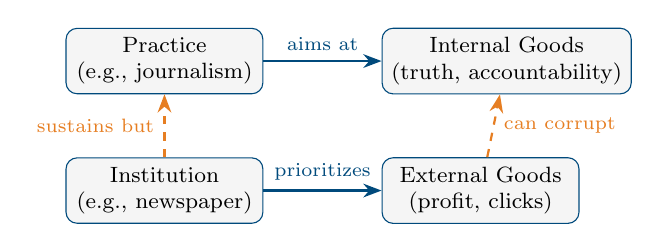
\begin{tikzpicture}[
        node distance=1.2cm,
        box/.style={rectangle, draw=primaryblue, fill=lightgray, rounded corners, minimum width=2.5cm, minimum height=0.8cm, align=center, font=\footnotesize},
        arrow/.style={-{Stealth}, thick, primaryblue}
    ]
        \node[box] (practice) {Practice\\(e.g., journalism)};
        \node[box, right=1.5cm of practice] (internal) {Internal Goods\\(truth, accountability)};
        \node[box, below=0.8cm of practice] (institution) {Institution\\(e.g., newspaper)};
        \node[box, right=1.5cm of institution] (external) {External Goods\\(profit, clicks)};
        
        \draw[arrow] (practice) -- node[above, font=\scriptsize] {aims at} (internal);
        \draw[arrow] (institution) -- node[above, font=\scriptsize] {prioritizes} (external);
        \draw[arrow, dashed, accentorange] (institution) -- node[left, font=\scriptsize] {sustains but} (practice);
        \draw[arrow, dashed, accentorange] (external) -- node[right, font=\scriptsize] {can corrupt} (internal);
    \end{tikzpicture}
    \end{center}
\end{frame}

%------------------------------------------------------
% SLIDE 19: Why Virtue Ethics for Technology?
%------------------------------------------------------
\begin{frame}{Why Virtue Ethics for Technology?}
    \begin{itemize}
        \item Rules-based ethics struggles with technology because innovation constantly creates situations no rule anticipated---virtue ethics asks what a wise person would do.
        \item Consequentialist calculations are difficult when effects are unpredictable, distributed across millions of users, and unfold over decades.
        \item Virtue ethics focuses on \textbf{character formation}: technologies shape our habits, and habits shape who we become---this is precisely what virtue ethics addresses.
        \item The virtue tradition emphasizes \textbf{practical wisdom} (phronesis)---the ability to navigate novel situations wisely---which is exactly what digital life demands.
    \end{itemize}
    
    \vspace{0.2em}
    
    \begin{center}
        \scriptsize
    \renewcommand{\arraystretch}{1.15}
    \begin{tabular}{>{\raggedright}p{3cm} >{\raggedright\arraybackslash}p{8.5cm}}
        \toprule
        \textbf{Challenge} & \textbf{Why Virtue Ethics Helps} \\
        \midrule
        Rapid change & Focus on character, not outdated rules \\
        Unpredictable effects & Cultivate wisdom for novel situations \\
        Habit formation & Directly addresses how practices shape character \\
        Relational complexity & Care ethics and Confucianism emphasize relationships \\
        Loss of community & Communitarianism diagnoses fragmentation \\
        \bottomrule
    \end{tabular}
    \end{center}
\end{frame}

%------------------------------------------------------
% SLIDE 20: Discussion Questions: Virtue Ethics Foundations
%------------------------------------------------------
\begin{frame}{Discussion Questions: Virtue Ethics Foundations}
    \begin{enumerate}
        \item Aristotle says we become what we repeatedly do. What character traits are your daily technology habits cultivating? Are these the traits you want to have?
        
        \vspace{0.5em}
        
        \item  What might the ``virtuous mean'' look like for smartphone use---avoiding both the excess of constant connection and the deficiency of total disconnection?
        
        \vspace{0.5em}
        
        \item  Confucian ethics emphasizes fulfilling roles in relationships. How does technology help or hinder your ability to be a good friend, child, sibling, or citizen?
        
        \vspace{0.5em}
        
        \item Think of an activity you care about (music, sports, art, learning). How do social media platforms affect whether you pursue its internal goods (excellence) or external goods (likes, followers)?
    \end{enumerate}
\end{frame}

%------------------------------------------------------
% SLIDE 21: Shannon Vallor: Technology and the Virtues
%------------------------------------------------------
\begin{frame}{Shannon Vallor: Technology and the Virtues}
    \begin{itemize}
        \item \textbf{Shannon Vallor} is a philosopher of technology at the Edinburgh Futures Institute; her book \textit{Technology and the Virtues} (2016) applies virtue ethics to emerging technologies.
        \item Vallor argues that we face a \textbf{technosocial condition}: technology and society co-evolve so rapidly that traditional moral frameworks struggle to keep pace.
        \item She synthesizes Aristotelian, Confucian, and Buddhist virtue traditions to develop a framework of \textbf{technomoral virtues}---character traits needed to flourish with technology.
        \item Her central claim: we cannot rely on rules or calculations alone; we need cultivated \textbf{practical wisdom} to navigate technological life well.
    \end{itemize}
    
    \vspace{0.3em}
    
    \begin{block}{Shannon Vallor, \textit{Technology and the Virtues} (2016)}
        ``Virtue ethics asks not `What should I do?' but `What kind of person should I become, and how?'---questions essential for beings whose characters are increasingly shaped by technological habits.''
    \end{block}
\end{frame}

%------------------------------------------------------
% SLIDE 22: Vallor's Twelve Technomoral Virtues
%------------------------------------------------------
\begin{frame}{Vallor's Twelve Technomoral Virtues}
    \begin{itemize}
        \item Vallor identifies \textbf{twelve technomoral virtues} that draw on multiple traditions and address the specific challenges of life with emerging technologies.
        \item These virtues are not new inventions but classical virtues \textbf{reinterpreted} for contexts shaped by social media, AI, surveillance, and global connectivity.
        \item The list culminates in \textbf{technomoral wisdom}---the integrating virtue that enables us to apply all others appropriately in novel technological situations.
        \item Vallor emphasizes that these virtues must be \textbf{cultivated through practice}---they cannot be downloaded or installed like software.
    \end{itemize}
    
    \vspace{0.2em}
    
    \begin{center}
    \renewcommand{\arraystretch}{1.1}
    \footnotesize
    \begin{tabular}{>{\raggedright}p{3.5cm} >{\raggedright}p{3.5cm} >{\raggedright\arraybackslash}p{4.5cm}}
        \toprule
        \textbf{Self-Regarding} & \textbf{Other-Regarding} & \textbf{Integrating} \\
        \midrule
        Honesty & Empathy & Perspective \\
        Self-Control & Care & Magnanimity \\
        Humility & Civility & \textbf{Technomoral Wisdom} \\
        Courage & Justice & \\
        & Flexibility & \\
        \bottomrule
    \end{tabular}
    \end{center}
\end{frame}

%------------------------------------------------------
% SLIDE 23: Vallor's The AI Mirror (2024)
%------------------------------------------------------
\begin{frame}{Vallor's \textit{The AI Mirror} (2024)}
    \begin{itemize}
        \item In \textit{The AI Mirror} (2024), Vallor extends her framework to generative AI, arguing that AI is best understood as a \textbf{mirror}, not a mind.
        \item Just as a mirror reflects your image without containing a second face, AI systems reflect patterns from human data without possessing understanding or experience.
        \item Vallor warns that the greater danger is not superintelligent AI but \textbf{undermining our sense of ourselves} as responsible, reasoning, free intelligences.
        \item Silicon Valley promotes a ``debased version of what we are''---viewing humans as ``soft, wet computers''---which erodes our confidence in human wisdom and agency.
    \end{itemize}
    
    \vspace{0.3em}
    
    \begin{alertblock}{The Mirror Metaphor}
        ``When you look in a mirror, you know there isn't a second face looking back at you from the other side of the glass. That's just a reflection of your face. There's nothing on the other side participating.''
    \end{alertblock}
\end{frame}

%------------------------------------------------------
% SLIDE 24: Vallor on AI and Human Wisdom
%------------------------------------------------------
\begin{frame}{Vallor on AI and Human Wisdom}
    \begin{itemize}
        \item Vallor critiques the redefinition of intelligence to mean ``performing economically valuable tasks''---this conflates competence with genuine understanding.
        \item Large language models do not truly reason; they ``bullshit a whole chain of thought'' that can collapse into nonsense when pressed---mimicry without comprehension.
        \item \textbf{Thinking requires experience}: ``Thinking without experience is like water without hydrogen---you've taken something out that loses its identity.''
        \item Yet Vallor remains hopeful: technology at its core \textit{can} be humane---``We're at a moment when we need to rebuild our confidence in the capabilities of humans to reason wisely.''
    \end{itemize}
    
    \vspace{0.2em}
    
    \begin{center}
    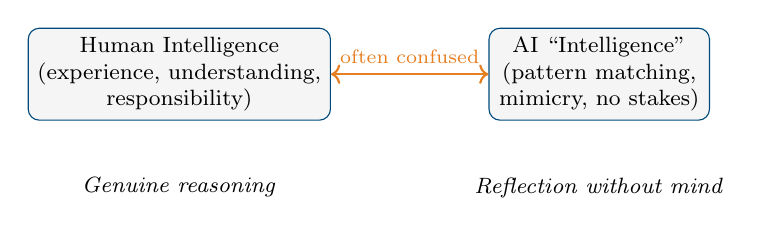
\begin{tikzpicture}[
        node distance=1.5cm,
        box/.style={rectangle, draw=primaryblue, fill=lightgray, rounded corners, minimum width=2.8cm, minimum height=0.9cm, align=center, font=\footnotesize}
    ]
        \node[box] (human) {Human Intelligence\\(experience, understanding,\\responsibility)};
        \node[box, right=2cm of human] (ai) {AI ``Intelligence''\\(pattern matching,\\mimicry, no stakes)};
        \node[draw=none, below=0.6cm of human] (hlabel) {\footnotesize\textit{Genuine reasoning}};
        \node[draw=none, below=0.6cm of ai] (alabel) {\footnotesize\textit{Reflection without mind}};
        
        \draw[thick, accentorange, <->] (human) -- node[above, font=\scriptsize] {often confused} (ai);
    \end{tikzpicture}
    \end{center}
\end{frame}

%------------------------------------------------------
% SLIDE 25: Sherry Turkle: Alone Together
%------------------------------------------------------
\begin{frame}{Sherry Turkle: Alone Together}
    \begin{itemize}
        \item \textbf{Sherry Turkle} is a psychologist and professor at MIT who has studied human-technology relationships for over forty years.
        \item In \textit{Alone Together} (2011), Turkle documents a troubling paradox: we are increasingly \textbf{connected} through devices but increasingly \textbf{alone} in meaningful human contact.
        \item She observes a ``flight from conversation'': people prefer texting to talking, curated posts to spontaneous interaction, and controllable digital exchanges to unpredictable face-to-face encounters.
        \item Turkle warns that we are designing technologies that offer the \textbf{illusion of companionship} without the demands of real relationship.
    \end{itemize}
    
    \vspace{0.3em}
    
    \begin{block}{Sherry Turkle, \textit{Alone Together} (2011)}
        ``We expect more from technology and less from each other... We are tempted to think that our little `sips' of online connection add up to a big gulp of real conversation. But they don't.''
    \end{block}
\end{frame}

%------------------------------------------------------
% SLIDE 26: Turkle: Reclaiming Conversation
%------------------------------------------------------
\begin{frame}{Turkle: Reclaiming Conversation}
    \begin{itemize}
        \item In \textit{Reclaiming Conversation} (2015), Turkle argues that face-to-face conversation is the most humanizing thing we do---and we are systematically abandoning it.
        \item Conversation develops \textbf{empathy}: children learn to read faces, tolerate ambiguity, and respond to others' emotions through unstructured talk, not screens.
        \item Turkle identifies the importance of \textbf{solitude}---the capacity to be alone with one's thoughts---which is eroded when we reach for phones at every moment of boredom.
        \item She calls for reclaiming ``sacred spaces'' for conversation: the kitchen table, the dining room, the car, the classroom---places where phones should not intrude.
    \end{itemize}
    
    \vspace{0.2em}
    
    \begin{center}
    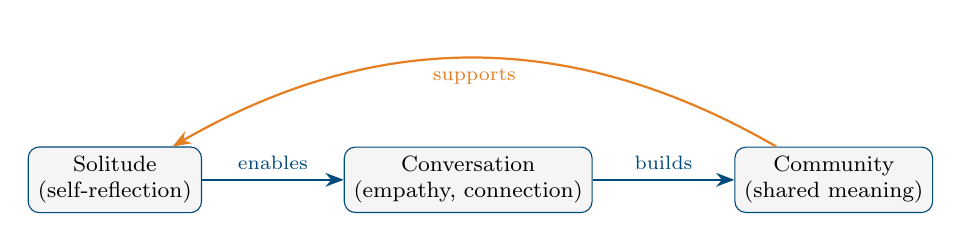
\begin{tikzpicture}[
        node distance=1.8cm,
        box/.style={rectangle, draw=primaryblue, fill=lightgray, rounded corners, minimum width=2.2cm, minimum height=0.7cm, align=center, font=\footnotesize}
    ]
        \node[box] (solitude) {Solitude\\(self-reflection)};
        \node[box, right=of solitude] (conversation) {Conversation\\(empathy, connection)};
        \node[box, right=of conversation] (community) {Community\\(shared meaning)};
        
        \draw[-{Stealth}, thick, primaryblue] (solitude) -- node[above, font=\scriptsize] {enables} (conversation);
        \draw[-{Stealth}, thick, primaryblue] (conversation) -- node[above, font=\scriptsize] {builds} (community);
        \draw[-{Stealth}, thick, accentorange, bend right=30] (community) to node[below, font=\scriptsize] {supports} (solitude);
    \end{tikzpicture}
    \end{center}
\end{frame}

%------------------------------------------------------
% SLIDE 27: Turkle on Artificial Intimacy (2024)
%------------------------------------------------------
\begin{frame}{Turkle on Artificial Intimacy (2024)}
    \begin{itemize}
        \item In her 2024 preface to \textit{Reclaiming Conversation}, Turkle extends her analysis to AI chatbots that simulate emotional connection and understanding.
        \item She argues that social media was our \textbf{gateway drug}: it trained us to accept mediated relationships, preparing us for ``conversations'' with machines.
        \item AI companions offer \textbf{frictionless relationships}---always available, never demanding, endlessly patient---but this convenience comes at a cost.
        \item Turkle invokes psychoanalyst Erik Erikson's warning about engineers who ``aren't convinced that people have an interior''---reducing humans to information processors.
    \end{itemize}
    
    \vspace{0.3em}
    
    \begin{alertblock}{The Problem of Unrequited Love}
        ``We nurture what we love, but we love what we nurture. We love what we allow ourselves to relate to. It's important to remember that this love is unrequited.''
    \end{alertblock}
\end{frame}

%------------------------------------------------------
% SLIDE 28: Turkle: What Machines Cannot Provide
%------------------------------------------------------
\begin{frame}{Turkle: What Machines Cannot Provide}
    \begin{itemize}
        \item Turkle challenges the view (held by figures like Eric Schmidt) that AI with access to ``every paper on anxiety'' could replace human therapists or friends.
        \item Information is not understanding: ``When you tell your troubles to a machine, it has no stake in the conversation. It can't feel pain. It has no life in which you play a part.''
        \item The \textbf{performance of emotion} does not make machines more human---but it does challenge what we think makes \textit{people} special.
        \item Drawing on philosopher Emmanuel Levinas, Turkle emphasizes that the \textbf{human face} initiates an ethical compact---embodied presence creates obligations that screens cannot.
    \end{itemize}
    
    \vspace{0.2em}
    
    \begin{exampleblock}{The Levinas Point}
        For Levinas, encountering another person's face creates an immediate ethical demand: ``Here I am, responsible for you.'' A chatbot has no face, no vulnerability, no mortality---and thus makes no genuine ethical claim on us, nor we on it.
    \end{exampleblock}
\end{frame}

%------------------------------------------------------
% SLIDE 29: Luciano Floridi: Five Principles for AI Ethics
%------------------------------------------------------
\begin{frame}{Luciano Floridi: Five Principles for AI Ethics}
    \begin{itemize}
        \item \textbf{Luciano Floridi} is a philosopher at Yale and Oxford who developed the concepts of the ``infosphere'' and ``inforgs'' we encountered earlier.
        \item In his ``Unified Framework of Five Principles for AI in Society'' (2019), Floridi analyzed 47 AI ethics documents and found convergence around \textbf{five core principles}.
        \item Four principles come from \textbf{bioethics}: beneficence (do good), non-maleficence (avoid harm), autonomy (respect human choice), and justice (be fair).
        \item Floridi adds a fifth principle specific to AI: \textbf{explicability}---combining intelligibility (``How does it work?'') with accountability (``Who is responsible?'').
    \end{itemize}
    
    \vspace{0.2em}
    
    \begin{center}
    \renewcommand{\arraystretch}{1.15}
    \scriptsize
    \begin{tabular}{>{\raggedright}p{2.8cm} >{\raggedright\arraybackslash}p{8.5cm}}
        \toprule
        \textbf{Principle} & \textbf{Core Question} \\
        \midrule
        Beneficence & Does this AI promote human wellbeing and flourishing? \\
        Non-maleficence & Does this AI avoid causing harm to individuals or society? \\
        Autonomy & Does this AI respect and preserve human decision-making? \\
        Justice & Does this AI treat people fairly and avoid discrimination? \\
        \textbf{Explicability} & Can we understand how it works and who is responsible? \\
        \bottomrule
    \end{tabular}
    \end{center}
\end{frame}

%------------------------------------------------------
% SLIDE 30: Floridi: AI as Agency Without Intelligence
%------------------------------------------------------
\begin{frame}{Floridi: AI as Agency Without Intelligence}
    \begin{itemize}
        \item Floridi describes AI as ``smart agency on tap''---systems that can \textbf{act} in the world (book flights, filter content, recommend products) without genuine understanding.
        \item This is \textbf{agency without intelligence}: AI systems produce effects and make consequential decisions, but they don't ``know'' what they're doing in any meaningful sense.
        \item The ethical challenge is that we are delegating more decisions to systems that cannot be held responsible, understand context, or exercise moral judgment.
        \item Floridi's explicability principle responds to this: if AI acts without understanding, \textit{humans} must understand how it works and remain accountable for its effects.
    \end{itemize}
    
    \vspace{0.3em}
    
    \begin{block}{The Explicability Gap}
        Many AI systems are ``black boxes'': even their creators cannot fully explain why they produce particular outputs. This creates an \textbf{explicability gap} that threatens accountability---if no one understands how a decision was made, who is responsible when it causes harm?
    \end{block}
\end{frame}

%------------------------------------------------------
% SLIDE 31: Jonathan Haidt: The Anxious Generation
%------------------------------------------------------
\begin{frame}{Jonathan Haidt: The Anxious Generation}
    \begin{itemize}
        \item \textbf{Jonathan Haidt} is a social psychologist at NYU whose book \textit{The Anxious Generation} (2024) argues that smartphones and social media have caused a mental health crisis among youth.
        \item Haidt identifies \textbf{four foundational harms} of phone-based childhood: social deprivation, sleep deprivation, attention fragmentation, and addiction.
        \item The shift from ``play-based childhood'' to ``phone-based childhood'' (roughly 2010--2015) correlates with sharp increases in anxiety, depression, and self-harm among adolescents.
        \item Haidt proposes concrete reforms: no smartphones before high school, no social media before 16, phone-free schools, and more unsupervised outdoor play.
    \end{itemize}
    
    \vspace{0.2em}
    
    \begin{center}
    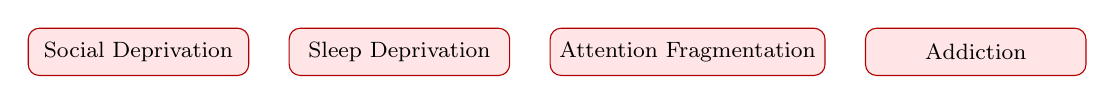
\begin{tikzpicture}[
        node distance=0.6cm,
        harm/.style={rectangle, draw=red!70!black, fill=red!10, rounded corners, minimum width=2.8cm, minimum height=0.6cm, align=center, font=\footnotesize}
    ]
        \node[harm] (social) {Social Deprivation};
        \node[harm, right=0.5cm of social] (sleep) {Sleep Deprivation};
        \node[harm, right=0.5cm of sleep] (attention) {Attention Fragmentation};
        \node[harm, right=0.5cm of attention] (addiction) {Addiction};
    \end{tikzpicture}
    \end{center}
\end{frame}

%------------------------------------------------------
% SLIDE 32: Haidt on AI: Amplifying Existing Harms
%------------------------------------------------------
\begin{frame}{Haidt on AI: Amplifying Existing Harms}
    \begin{itemize}
        \item In a 2023 essay with Eric Schmidt, Haidt argues that AI is ``about to make social media much more toxic''---not a separate problem but an \textbf{amplifier of existing harms}.
        \item Haidt identifies four imminent AI threats: super-empowering bad actors, drowning in fake evidence (deepfakes), accelerating polarization, and enabling new forms of harassment.
        \item AI companions pose particular risks for young people: chatbots designed to simulate friendship and intimacy may further displace real human relationships.
        \item Haidt's analysis shows \textbf{continuity}: the same dynamics that made social media harmful (attention capture, social comparison, displacement of real connection) are intensified by AI.
    \end{itemize}
    
    \vspace{0.3em}
    
    \begin{alertblock}{Haidt and Schmidt (2023)}
        ``Generative AI is going to pour gasoline on the fire of social media's harms... The same business model---capturing attention and selling it to advertisers---will now deploy far more powerful tools to keep users engaged.''
    \end{alertblock}
\end{frame}

%------------------------------------------------------
% SLIDE 33: Critics of Haidt: The Evidence Debate
%------------------------------------------------------
\begin{frame}{Critics of Haidt: The Evidence Debate}
    \begin{itemize}
        \item Haidt's claims have provoked significant scholarly debate; critics argue the evidence for social media causing mental health harms is weaker than he suggests.
        \item \textbf{Candice Odgers} (UC Irvine) argues that correlations between screen time and mental health are small and inconsistent, and that Haidt overstates causation.
        \item \textbf{Amy Orben} (Cambridge) notes that effect sizes in studies are often tiny---comparable to the ``harm'' of eating potatoes---and that moral panic may cause its own harms.
        \item The debate matters: if Haidt is wrong, we may restrict beneficial technologies; if critics are wrong, we may fail to protect vulnerable youth from genuine harm.
    \end{itemize}
    
    \vspace{0.2em}
    
    \begin{center}
        \scriptsize
    \renewcommand{\arraystretch}{1.15}
    \begin{tabular}{>{\raggedright}p{5.5cm} >{\raggedright\arraybackslash}p{5.5cm}}
        \toprule
        \textbf{Haidt's Position} & \textbf{Critics' Response} \\
        \midrule
        Strong causal link to mental health crisis & Correlations are small and inconsistent \\
        Smartphones are the key variable & Many factors changed simultaneously \\
        Urgent action needed now & Moral panic may cause its own harms \\
        Natural experiments support causation & Methodological concerns with studies \\
        \bottomrule
    \end{tabular}
    \end{center}
\end{frame}

%------------------------------------------------------
% SLIDE 34: Social Media and Political Polarization
%------------------------------------------------------
\begin{frame}{Social Media and Political Polarization}
    \begin{itemize}
        \item Social media platforms have been accused of driving \textbf{political polarization}---the widening gap between political groups and the increasing hostility between them.
        \item \textbf{Filter bubbles} and algorithmic curation may expose users primarily to views they already hold, making opposing views seem extreme or incomprehensible.
        \item \textbf{Outrage amplification}: content that provokes anger and moral outrage generates more engagement, so algorithms systematically promote divisive content.
        \item The shift from broadcast media (shared national conversation) to personalized feeds means citizens increasingly live in \textbf{different information worlds}.
    \end{itemize}
    
    \vspace{0.2em}
    
    \begin{center}
    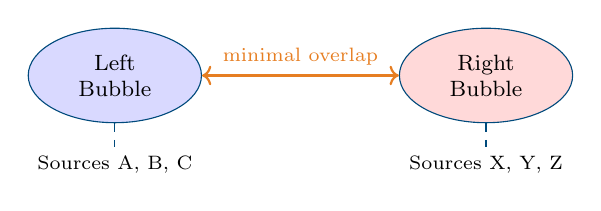
\begin{tikzpicture}[
        node distance=1cm,
        bubble/.style={ellipse, draw=primaryblue, fill=lightgray, minimum width=2.2cm, minimum height=1.2cm, align=center, font=\footnotesize}
    ]
        \node[bubble, fill=blue!15] (left) {Left\\Bubble};
        \node[bubble, fill=red!15, right=2.5cm of left] (right) {Right\\Bubble};
        \node[draw=none, below=0.3cm of left] (lsource) {\scriptsize Sources A, B, C};
        \node[draw=none, below=0.3cm of right] (rsource) {\scriptsize Sources X, Y, Z};
        
        \draw[thick, accentorange, <->] (left) -- node[above, font=\scriptsize] {minimal overlap} (right);
        \draw[dashed, primaryblue] (left) -- (lsource);
        \draw[dashed, primaryblue] (right) -- (rsource);
    \end{tikzpicture}
    \end{center}
\end{frame}

%------------------------------------------------------
% SLIDE 35: The Erosion of Shared Reality
%------------------------------------------------------
\begin{frame}{The Erosion of Shared Reality}
    \begin{itemize}
        \item Political philosopher \textbf{Hannah Arendt} argued that democratic life requires a \textbf{common world}---shared facts and frameworks that allow citizens to disagree productively.
        \item Social media threatens this common world: when groups cannot agree on basic facts, democratic deliberation becomes impossible.
        \item \textbf{Deepfakes} and AI-generated content accelerate this erosion---soon any image, video, or audio can be fabricated, making ``seeing is believing'' obsolete.
        \item The result is not that everyone believes lies, but that \textbf{no one believes anything}---a cynicism that benefits those who prefer citizens disengaged and confused.
    \end{itemize}
    
    \vspace{0.3em}
    
    \begin{block}{Hannah Arendt, \textit{The Origins of Totalitarianism} (1951)}
        ``The ideal subject of totalitarian rule is not the convinced Nazi or the convinced Communist, but people for whom the distinction between fact and fiction... no longer exist[s].''
    \end{block}
\end{frame}

%------------------------------------------------------
% SLIDE 36: Virtue and Democratic Citizenship
%------------------------------------------------------
\begin{frame}{Virtue and Democratic Citizenship}
    \begin{itemize}
        \item Democratic self-government requires \textbf{civic virtues}: the character traits that enable citizens to participate thoughtfully in collective decision-making.
        \item Classical republicans emphasized virtues like \textbf{public-spiritedness} (concern for common good over private interest), \textbf{deliberative openness} (willingness to hear other views), and \textbf{civic courage} (speaking truth even when unpopular).
        \item Social media may erode these virtues: rewarding performance over deliberation, tribalism over public-spiritedness, and outrage over thoughtful engagement.
        \item The question is not just ``Is social media making us unhappy?'' but ``Is it making us \textbf{worse citizens}?''
    \end{itemize}
    
    \vspace{0.2em}
    
    \begin{center}
        \scriptsize
    \renewcommand{\arraystretch}{1.15}
    \begin{tabular}{>{\raggedright}p{3.5cm} >{\raggedright\arraybackslash}p{7.5cm}}
        \toprule
        \textbf{Civic Virtue} & \textbf{How Social Media May Erode It} \\
        \midrule
        Public-spiritedness & Algorithms reward tribal loyalty over common good \\
        Deliberative openness & Filter bubbles limit exposure to other views \\
        Civic courage & Pile-ons and cancellation punish dissent \\
        Truthfulness & Engagement metrics reward sensationalism \\
        \bottomrule
    \end{tabular}
    \end{center}
\end{frame}

%------------------------------------------------------
% SLIDE 37: AI as the Next Chapter in the Same Story
%------------------------------------------------------
\begin{frame}{AI as the Next Chapter in the Same Story}
    \begin{itemize}
        \item The arrival of generative AI (ChatGPT, November 2022) is not a break from the social media era but its \textbf{continuation and intensification}.
        \item The same dynamics apply: attention capture, engagement optimization, displacement of human connection, and the erosion of skills we once cultivated.
        \item What social media did to our \textit{social} lives---fragmenting attention, encouraging performance, substituting metrics for meaning---AI threatens to do to our \textit{intellectual} lives.
        \item All four thinkers we've studied see this continuity: Vallor (technomoral virtues still needed), Turkle (gateway drug), Haidt (gasoline on fire), Floridi (agency without intelligence).
    \end{itemize}
    
    \vspace{0.2em}
    
    \begin{center}
    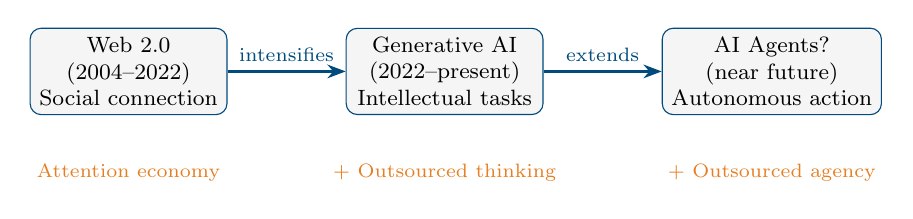
\begin{tikzpicture}[
        node distance=0.8cm,
        era/.style={rectangle, draw=primaryblue, fill=lightgray, rounded corners, minimum width=2.5cm, minimum height=1cm, align=center, font=\footnotesize},
        arrow/.style={-{Stealth}, thick, primaryblue}
    ]
        \node[era] (web2) {Web 2.0\\(2004--2022)\\Social connection};
        \node[era, right=1.5cm of web2] (ai) {Generative AI\\(2022--present)\\Intellectual tasks};
        \node[era, right=1.5cm of ai] (future) {AI Agents?\\(near future)\\Autonomous action};
        
        \draw[arrow] (web2) -- node[above, font=\scriptsize] {intensifies} (ai);
        \draw[arrow] (ai) -- node[above, font=\scriptsize] {extends} (future);
        
        \node[draw=none, below=0.5cm of web2, font=\scriptsize, text=accentorange] {Attention economy};
        \node[draw=none, below=0.5cm of ai, font=\scriptsize, text=accentorange] {+ Outsourced thinking};
        \node[draw=none, below=0.5cm of future, font=\scriptsize, text=accentorange] {+ Outsourced agency};
    \end{tikzpicture}
    \end{center}
\end{frame}

%------------------------------------------------------
% SLIDE 38: AI and the Virtue of Honesty
%------------------------------------------------------
\begin{frame}{AI and the Virtue of Honesty}
    \begin{itemize}
        \item \textbf{Honesty} is a core virtue in every tradition we've studied---Aristotle's truthfulness, Confucian sincerity, religious commands against bearing false witness.
        \item Generative AI makes deception radically easier: \textbf{deepfakes} can fabricate video of anyone saying anything; AI can generate convincing fake news at scale.
        \item But there's a subtler threat: AI-generated content blurs the line between human and machine authorship---is submitting AI-written work as your own a form of dishonesty?
        \item Vallor's technomoral honesty requires ``habitually presenting oneself and one's work accurately''---a virtue increasingly difficult to practice and verify in an AI-saturated world.
    \end{itemize}
    
    \vspace{0.3em}
    
    \begin{alertblock}{The Authenticity Question}
        When you read a heartfelt social media post, how do you know a human wrote it? When you receive a personalized message, how do you know someone actually composed it for you? AI threatens not just truth but \textbf{authenticity}---the connection between expression and genuine human intention.
    \end{alertblock}
\end{frame}

%------------------------------------------------------
% SLIDE 39: AI and the Intellectual Virtues
%------------------------------------------------------
\begin{frame}{AI and the Intellectual Virtues}
    \begin{itemize}
        \item The \textbf{intellectual virtues}---curiosity, careful reasoning, intellectual humility, love of truth---are capacities developed through practice and struggle.
        \item If AI can instantly produce essays, solve problems, and answer questions, what happens to the \textbf{habits of mind} we develop by doing these things ourselves?
        \item There's a parallel to GPS navigation: convenient, but studies show heavy GPS users develop weaker spatial reasoning and memory for routes.
        \item The question is not whether AI is useful (it obviously can be) but whether outsourcing intellectual labor \textbf{atrophies the virtues} that labor was meant to cultivate.
    \end{itemize}
    
    \vspace{0.2em}
    
    \begin{exampleblock}{The Student's Dilemma}
        A student can use AI to write an essay in minutes. But the assignment existed to develop skills: organizing thoughts, constructing arguments, expressing ideas clearly. If AI does the work, the student gets the grade but misses the growth. What virtue would help navigate this tension?
    \end{exampleblock}
\end{frame}

%------------------------------------------------------
% SLIDE 40: AI and the Relational Virtues
%------------------------------------------------------
\begin{frame}{AI and the Relational Virtues}
    \begin{itemize}
        \item \textbf{Relational virtues}---empathy, care, compassion, fidelity---are cultivated through relationships with other humans who have their own needs, perspectives, and vulnerabilities.
        \item AI companions offer relationships without friction: they never get tired, never disagree, never have needs of their own---but this ``ease'' may prevent virtue development.
        \item Recall Turkle: ``When you tell your troubles to a machine, it has no stake in the conversation. It can't feel pain. It has no life in which you play a part.''
        \item And Vallor: there is ``nothing on the other side participating''---the reciprocity that makes human relationships both difficult and morally formative is absent.
    \end{itemize}
    
    \vspace{0.2em}
    
    \begin{center}
        \scriptsize
    \renewcommand{\arraystretch}{1.15}
    \begin{tabular}{>{\raggedright}p{4cm} >{\raggedright}p{3.5cm} >{\raggedright\arraybackslash}p{3.5cm}}
        \toprule
        \textbf{Feature} & \textbf{Human Relationship} & \textbf{AI Companion} \\
        \midrule
        Availability & Limited, scheduled & Always on demand \\
        Reciprocity & Mutual needs and care & One-directional \\
        Friction & Disagreement, conflict & Designed to please \\
        Stakes & Real consequences & No genuine stakes \\
        \bottomrule
    \end{tabular}
    \end{center}
\end{frame}

%------------------------------------------------------
% SLIDE 41: AI and Human Agency
%------------------------------------------------------
\begin{frame}{AI and Human Agency}
    \begin{itemize}
        \item For Aristotle, virtue requires \textbf{prohairesis}---deliberate choice---which is why we don't praise or blame people for involuntary actions or accidents.
        \item AI systems increasingly make choices that affect our lives: what content we see, which job applicants advance, what medical treatments are recommended.
        \item When AI makes decisions, \textbf{human agency is displaced}: we become subjects of algorithmic governance rather than authors of our own choices.
        \item Floridi's \textbf{autonomy principle} insists that AI should preserve and enhance human decision-making, not replace it---but current systems often do the opposite.
    \end{itemize}
    
    \vspace{0.2em}
    
    \begin{center}
    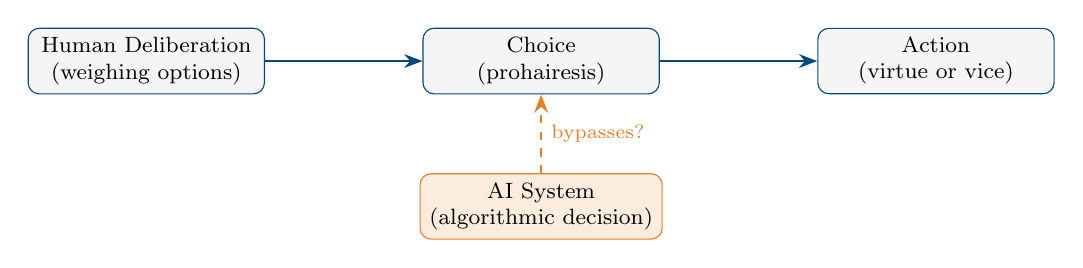
\begin{tikzpicture}[
        node distance=1.2cm,
        box/.style={rectangle, draw=primaryblue, fill=lightgray, rounded corners, minimum width=3cm, minimum height=0.8cm, align=center, font=\footnotesize},
        arrow/.style={-{Stealth}, thick}
    ]
        \node[box] (human) {Human Deliberation\\(weighing options)};
        \node[box, right=2cm of human] (choice) {Choice\\(prohairesis)};
        \node[box, right=2cm of choice] (action) {Action\\(virtue or vice)};
        
        \draw[arrow, primaryblue] (human) -- (choice);
        \draw[arrow, primaryblue] (choice) -- (action);
        
        \node[box, below=1cm of choice, draw=accentorange, fill=accentorange!15] (ai) {AI System\\(algorithmic decision)};
        \draw[arrow, accentorange, dashed] (ai) -- node[right, font=\scriptsize] {bypasses?} (choice);
    \end{tikzpicture}
    \end{center}
\end{frame}

%------------------------------------------------------
% SLIDE 42: Can AI Systems Be Virtuous?
%------------------------------------------------------
\begin{frame}{Can AI Systems Be Virtuous?}
    \begin{itemize}
        \item Some argue we should design AI systems to be ``virtuous''---to embody honesty, fairness, care---but can a machine \textit{possess} virtues in any meaningful sense?
        \item Aristotle's virtues require \textbf{feeling the right emotions} at the right time---courage involves feeling appropriate fear, not just acting bravely.
        \item Vallor argues that genuine thinking requires \textbf{experience}: ``Thinking without experience is like water without hydrogen---you've taken something out that loses its identity.''
        \item AI can \textit{simulate} virtuous behavior and produce outputs that \textit{look} virtuous, but simulation is not the same as genuine character.
    \end{itemize}
    
    \vspace{0.3em}
    
    \begin{block}{The Simulation Problem}
        An AI can be programmed to say kind things, but it cannot \textit{care}. It can produce fair-seeming outputs, but it has no \textit{commitment} to justice. Virtues are not just behaviors but stable dispositions rooted in understanding, emotion, and choice---things AI systems lack.
    \end{block}
\end{frame}

%------------------------------------------------------
% SLIDE 43: Vallor's Challenge: Collective Action
%------------------------------------------------------
\begin{frame}{Vallor's Challenge: Collective Action}
    \begin{columns}[T]
        \begin{column}{0.55\textwidth}
            \small
            \begin{itemize}
                \item Vallor argues that individual virtue is necessary but not sufficient---we also need \textbf{collective action} to reshape the technological environment itself.
                \item Personal discipline (limiting screen time, cultivating attention) helps, but platforms are \textit{designed} to undermine such discipline---willpower alone cannot win.
                \item We need structural changes: regulations that constrain harmful business models, design standards that respect human flourishing, and institutions that support virtue cultivation.
                \item This connects to communitarian insights: virtues are cultivated within communities and practices, not by isolated individuals resisting hostile environments.
            \end{itemize}
        \end{column}
        
        \begin{column}{0.4\textwidth}
            \begin{center}
            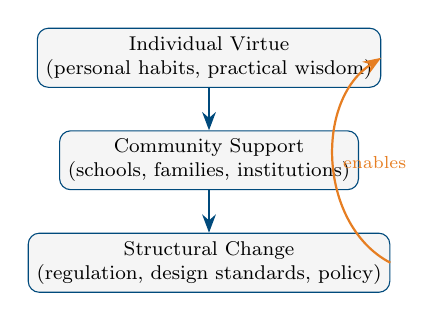
\begin{tikzpicture}[
                scale = 0.9,
                transform shape,
                node distance=0.8cm,
                level/.style={rectangle, draw=primaryblue, fill=lightgray, rounded corners, minimum width=3.5cm, minimum height=0.7cm, align=center, font=\footnotesize}
            ]
                \node[level] (individual) {Individual Virtue\\(personal habits, practical wisdom)};
                \node[level, below=0.6cm of individual] (community) {Community Support\\(schools, families, institutions)};
                \node[level, below=0.6cm of community] (structural) {Structural Change\\(regulation, design standards, policy)};
                
                \draw[-{Stealth}, thick, primaryblue] (individual) -- (community);
                \draw[-{Stealth}, thick, primaryblue] (community) -- (structural);
                \draw[-{Stealth}, thick, accentorange, bend left=60] (structural.east) to node[right, font=\scriptsize] {enables} (individual.east);
            \end{tikzpicture}
            \end{center}
        \end{column}
    \end{columns}
\end{frame}

%------------------------------------------------------
% SLIDE 44: Discussion Questions: Social Media, Politics, and AI
%------------------------------------------------------
\begin{frame}{Discussion Questions: Social Media, Politics, and AI}
    \begin{enumerate}
        \item  Haidt claims smartphones caused a mental health crisis; critics say the evidence is weak. How should we make policy when experts disagree? Should we err on the side of caution?
        
        \vspace{0.4em}
        
        \item  Arendt says democracy requires a ``common world'' of shared facts. Is this still possible in an age of personalized feeds and AI-generated content? What would it take to rebuild?
        
        \vspace{0.4em}
        
        \item If AI can write your essays and solve your problems, how do you develop the intellectual virtues those tasks were meant to cultivate? Is there a virtuous way to use AI for learning?
        
        \vspace{0.4em}
        
        \item Vallor says individual virtue isn't enough---we need structural change. But structural change requires political action, which requires virtuous citizens. How do we escape this circle?
    \end{enumerate}
\end{frame}

%------------------------------------------------------
% SLIDE 45: What Virtue Traditions Teach Us
%------------------------------------------------------
\begin{frame}{What Virtue Traditions Teach Us}
    \begin{itemize}
        \item \textbf{Aristotle} teaches that character is formed by habits---our repeated digital practices are shaping who we become, whether we intend it or not.
        \item \textbf{Confucius} reminds us that virtue is relational---we must ask how technology affects our ability to fulfill our roles and obligations to others.
        \item \textbf{Care ethics} emphasizes attention and responsiveness to particular others---qualities threatened by distraction and algorithmic mediation.
        \item \textbf{Communitarians} warn that virtues require supportive communities and practices---isolated individuals cannot cultivate character against hostile environments.
    \end{itemize}
    
    \vspace{0.2em}
    
    \begin{center}
    \renewcommand{\arraystretch}{1.15}
    \begin{tabular}{>{\raggedright}p{3cm} >{\raggedright\arraybackslash}p{8cm}}
        \toprule
        \textbf{Tradition} & \textbf{Key Insight for Digital Life} \\
        \midrule
        Aristotelian & Habits form character; choose digital habits wisely \\
        Confucian & Virtue is relational; technology affects all our roles \\
        Care Ethics & Attention to particular others requires presence \\
        Communitarian & We need communities that support virtue cultivation \\
        \bottomrule
    \end{tabular}
    \end{center}
\end{frame}

%------------------------------------------------------
% SLIDE 46: Virtues for the Digital Age
%------------------------------------------------------
\begin{frame}{Virtues for the Digital Age}
    \begin{itemize}
        \item The classical virtues remain essential---honesty, courage, justice, practical wisdom---but our technological context gives them new applications and urgency.
        \item \textbf{Attention} emerges as a crucial virtue: the capacity to focus, to be present, to resist the constant pull of notifications and feeds.
        \item \textbf{Patience} and \textbf{tolerance for friction} counter the demand for instant gratification---meaningful things often require sustained effort and discomfort.
        \item \textbf{Humility} about our own knowledge becomes vital when AI can produce confident-sounding nonsense and filter bubbles confirm our biases.
    \end{itemize}
    
    \vspace{0.2em}
    
    \begin{center}
    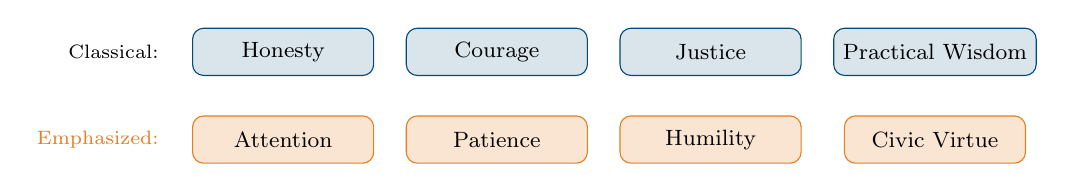
\begin{tikzpicture}[
        node distance=0.5cm,
        virtue/.style={rectangle, draw=primaryblue, fill=primaryblue!15, rounded corners, minimum width=2.3cm, minimum height=0.6cm, align=center, font=\footnotesize}
    ]
        \node[virtue] (honesty) {Honesty};
        \node[virtue, right=0.4cm of honesty] (courage) {Courage};
        \node[virtue, right=0.4cm of courage] (justice) {Justice};
        \node[virtue, right=0.4cm of justice] (wisdom) {Practical Wisdom};
        
        \node[virtue, below=0.5cm of honesty, fill=accentorange!20, draw=accentorange] (attention) {Attention};
        \node[virtue, below=0.5cm of courage, fill=accentorange!20, draw=accentorange] (patience) {Patience};
        \node[virtue, below=0.5cm of justice, fill=accentorange!20, draw=accentorange] (humility) {Humility};
        \node[virtue, below=0.5cm of wisdom, fill=accentorange!20, draw=accentorange] (civic) {Civic Virtue};
        
        \node[draw=none, left=0.3cm of honesty, font=\scriptsize] {Classical:};
        \node[draw=none, left=0.3cm of attention, font=\scriptsize, text=accentorange] {Emphasized:};
    \end{tikzpicture}
    \end{center}
\end{frame}

%------------------------------------------------------
% SLIDE 47: Looking Ahead: Reclaiming Friction
%------------------------------------------------------
\begin{frame}{Looking Ahead: Reclaiming Friction}
    \begin{itemize}
        \item Emerging technologies---AI agents, brain-computer interfaces, immersive virtual worlds---will intensify the challenges we've discussed, not resolve them.
        \item The temptation will be to embrace ever more seamless, frictionless experiences---but friction is often where growth, meaning, and virtue are forged.
        \item Turkle calls us to reclaim ``sacred spaces'' for unmediated human connection: meals without phones, classrooms without screens, conversations without interruption.
        \item The goal is not to reject technology but to \textbf{use it wisely}---with the practical wisdom to know when convenience serves flourishing and when it undermines it.
    \end{itemize}
    
    \vspace{0.3em}
    
    \begin{block}{The Case for Friction}
        Learning is hard. Relationships are messy. Thinking takes time. Democracy requires patience. These difficulties are not bugs to be engineered away but \textbf{features} of a meaningful human life. The virtuous response to technology is not rejection but \textbf{wise integration}---preserving the friction that makes us grow.
    \end{block}
\end{frame}

%------------------------------------------------------
% SLIDE 48: Final Reflection: Who Do You Want to Become?
%------------------------------------------------------
\begin{frame}{Final Reflection: Who Do You Want to Become?}
    \begin{itemize}
        \item Virtue ethics asks not ``What should I do right now?'' but ``What kind of person am I becoming through my choices and habits?''
        \item Every time you reach for your phone, scroll a feed, ask an AI to write for you, or choose a screen over a face---you are forming your character.
        \item The thinkers we've studied---Vallor, Turkle, Haidt, Floridi---offer not despair but a challenge: to cultivate the wisdom our technological moment demands.
        \item The question is not whether to use technology, but \textbf{how to use it in ways that help you flourish} as the person you want to become.
    \end{itemize}
    
    \vspace{0.3em}
    
    \begin{exampleblock}{Questions for Reflection}
        \begin{enumerate}
            \item What digital habits do you have that you're proud of? Which ones concern you?
            \item What would ``technomoral wisdom'' look like in your daily life?
            \item What is one concrete change you could make this week to better align your technology use with the person you want to become?
        \end{enumerate}
    \end{exampleblock}
\end{frame}

\end{document}